\begin{itemize}
\item Planck: Es gibt keine periodisch arbeitende Maschine, die nichts anderes bewirkt, als einem Wärmereservoir Wärme zu entziehen und diese vollständig in Arbeit umzuwandeln.
\item Clausius: Es gibt keine periodisch arbeitende Maschine, die nichts anderes bewirkt, als Wärme von einem kälteren zu einem wärmeren Körper zu transportieren.
\end{itemize}
Man zeigt: Wäre die eine Aussage falsch, so wäre auch die andere falsch. Betrachtet werden zwei Reservoire mit $T_\text{w} > T_\text{k}$.

\textbf{Planck folgt aus Clausius.} Angenommen, es gäbe eine Maschine P, die Planck verletzt: Sie entzieht dem warmen Reservoir die Wärme $Q$ und wandelt sie vollständig in die Arbeit $W = Q$ um. Mit dieser Arbeit treiben wir eine ideale Wärmepumpe an, die dem kalten Reservoir die Wärme $Q_\text{k}$ entzieht und dem warmen Reservoir $Q_\text{k}+W$ zuführt.
\begin{center}
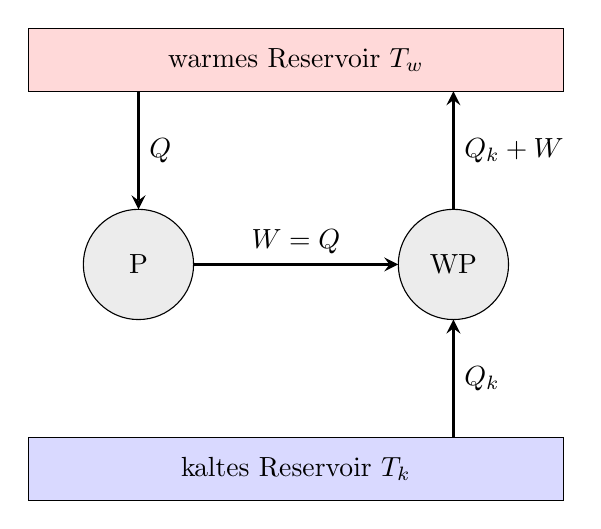
\begin{tikzpicture}[>=stealth]
 \draw[fill=red!15] (-3.4,2.2) rectangle (3.4,3.0);
 \node at (0,2.6) {warmes Reservoir $T_\text{w}$};
 \draw[fill=blue!15] (-3.4,-2.2) rectangle (3.4,-3.0);
 \node at (0,-2.6) {kaltes Reservoir $T_\text{k}$};
 \draw[fill=gray!15] (-2,0) circle (0.7);
 \node at (-2,0) {P};
 \draw[fill=gray!15] (2,0) circle (0.7);
 \node at (2,0) {WP};
 \draw[->, very thick] (-2,2.2) -- (-2,0.7) node[midway, right] {$Q$};
 \draw[->, very thick] (-1.3,0) -- (1.3,0) node[midway, above] {$W = Q$};
 \draw[->, very thick] (2,-2.2) -- (2,-0.7) node[midway, right] {$Q_\text{k}$};
 \draw[->, very thick] (2,0.7) -- (2,2.2) node[midway, right] {$Q_\text{k}+W$};
\end{tikzpicture}
\end{center}
Beide Maschinen zusammen arbeiten periodisch und bewirken nichts anderes, als dem kalten Reservoir die Wärme $Q_\text{k}$ zu entziehen und dem warmen Reservoir netto $Q_\text{k}+W-Q = Q_\text{k}$ zuzuführen. Das widerspricht Clausius. Gilt also Clausius, so gilt auch Planck.

\textbf{Clausius folgt aus Planck.} Angenommen, es gäbe eine Maschine C, die Clausius verletzt: Sie transportiert ohne Arbeit die Wärme $Q_\text{k}$ vom kalten zum warmen Reservoir. Zwischen den Reservoiren lassen wir einen idealen Stirlingmotor laufen, der dem warmen Reservoir die Wärme $Q_\text{w}$ entzieht, die Arbeit $W = Q_\text{w}-Q_\text{k}$ verrichtet und genau $Q_\text{k}$ an das kalte Reservoir abgibt.
\begin{center}
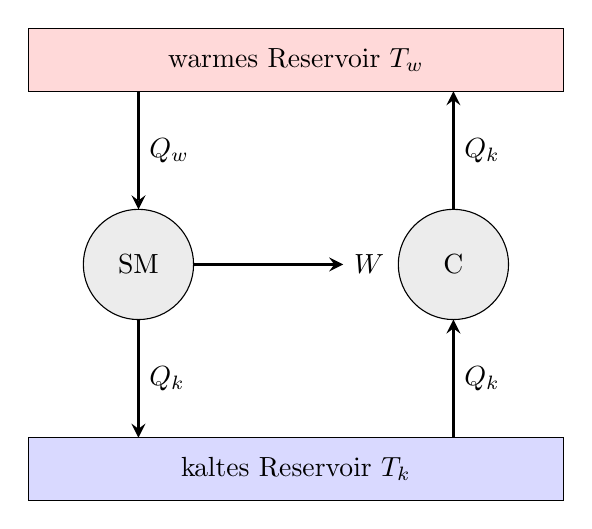
\begin{tikzpicture}[>=stealth]
 \draw[fill=red!15] (-3.4,2.2) rectangle (3.4,3.0);
 \node at (0,2.6) {warmes Reservoir $T_\text{w}$};
 \draw[fill=blue!15] (-3.4,-2.2) rectangle (3.4,-3.0);
 \node at (0,-2.6) {kaltes Reservoir $T_\text{k}$};
 \draw[fill=gray!15] (-2,0) circle (0.7);
 \node at (-2,0) {SM};
 \draw[fill=gray!15] (2,0) circle (0.7);
 \node at (2,0) {C};
 \draw[->, very thick] (-2,2.2) -- (-2,0.7) node[midway, right] {$Q_\text{w}$};
 \draw[->, very thick] (-2,-0.7) -- (-2,-2.2) node[midway, right] {$Q_\text{k}$};
 \draw[->, very thick] (-1.3,0) -- (0.6,0) node[right] {$W$};
 \draw[->, very thick] (2,-2.2) -- (2,-0.7) node[midway, right] {$Q_\text{k}$};
 \draw[->, very thick] (2,0.7) -- (2,2.2) node[midway, right] {$Q_\text{k}$};
\end{tikzpicture}
\end{center}
Das kalte Reservoir erhält gleich viel Wärme, wie ihm entzogen wird; es bleibt unverändert. Die beiden Maschinen zusammen entziehen also nur dem warmen Reservoir die Wärme $Q_\text{w}-Q_\text{k}$ und wandeln sie vollständig in die Arbeit $W$ um. Das widerspricht Planck. Gilt also Planck, so gilt auch Clausius.

Damit sind die beiden Formulierungen äquivalent.
